\section*{8/11}
\begin{center}
\underline{Численное интегрирование}
\end{center}
\[
\frac{\partial N_{\beta}}{\partial x} = J^{-1} \frac{\partial N_{\beta}}{\partial \xi}
\]

\underline{1. Формулы Ньютона-Котса}

$n$ точек, интерполяционный полином $(n+1)$-ого порядка, совпадающий в узлах с функцией $f(x)$ \\

\begin{center}
\begin{tikzpicture}
    \draw[->] (0,0) -- (7,0) node[below] {$x$};
    \draw[->] (0,0) -- (0,3.5) node[left] {$y$};

    \draw[domain=1:6.5, smooth, variable=\x, thick, blue, samples=300] 
        plot ({\x}, {sqrt(\x -1)+1});
        
    \node at (6, 3.7) {$f(x)$};
    
    \foreach \x in {1,2,3,4,5,6}
        \draw (\x,0.1) -- (\x,-0.1) ;
        
    \draw[dashed] (1, 0) -- (1, 1);
    \draw[dashed] (2, 0) -- (2, 2);
    \draw[dashed] (3, 0) -- (3, 2.4);
    \draw[dashed] (4, 0) -- (4, 2.7);
    \draw[dashed] (5, 0) -- (5, 3);
    \draw[dashed] (6, 0) -- (6, 3.2);
        
    \node at (1,-0.4) {$a$};
    \node at (6,-0.4) {$b$};
    
    \node at (-1, -1) {$n = 6$};
    \node at (3.5, -1) {\footnotesize $\displaystyle \Delta x = \frac{b-a}{5}$};

\end{tikzpicture}
\end{center}
\[
\int \limits_a^b f(x) dx = (b - a) \sum \limits_{i = 1}^n H_i \cdot f(x_i),
\]

где $H_i$ -- весовые коэффициенты

\begin{center}
\begin{tabular}{|c|c|}
\hline
$n = 2$ & \\
формула трапеции & \raisebox{1.5ex}[0cm][0cm] {$H_1 = \displaystyle \frac{1}{2},\ H_2 = \frac{1}{2}$}  \\
\hline
$n=3$ & \\
формула Симпсона & \raisebox{1.5ex}[0cm][0cm] {$H_1 = \displaystyle \frac{1}{6},\ H_2 = \frac{2}{3},\ H_3 = \frac{1}{6}$}  \\
\hline
& \\
\raisebox{1.5ex}[0cm][0cm] {$n=4$} & \raisebox{1.5ex}[0cm][0cm] {$H_1 = \displaystyle \frac{1}{8},\ H_2 = \frac{3}{8},\ H_3 = \frac{3}{8},\ H_4 = \frac{1}{8}$}  \\
\hline
& \\
\raisebox{1.5ex}[0cm][0cm] {$n=5$} & \raisebox{1.5ex}[0cm][0cm] {$H_1 = \displaystyle \frac{7}{90},\ H_2 = \frac{32}{90},\ H_3 = \frac{12}{90},\ H_4 = \frac{32}{90},\ H_5 = \frac{7}{90}$}  \\
\hline
\end{tabular}
\end{center}
\[
N_2(X) \text{ (2 -- порядок)},\ N^TN - \text{ 4 порядок},\ B^T B - \text{ 2 порядок}
\]
\newpage
\underline{2. Квадратурные формулы Гаусса-Лежандра}

$n$ точек, рассматриваем $2n$ неизвестных функций $f$ и $x$, $(2n-1)$ -- порядок интерполяционного многочлена.
\[
N^T N \Rightarrow 4 = 2n - 1,\ n = \frac{5}{2} = 2.5 \approx 3
\]

(для многочлена 4 порядка достаточно трех точек интегрирования)
\[
\int \limits_{-1}^1 f(\xi) d\xi = \sum \limits_{i = 1}^n f(\xi_i) H_i
\]

$n = 2:$
\begin{center}
\begin{tikzpicture}
    \draw[->] (0,0) -- (6,0) node[below] {$\xi$};

    \draw[domain=1:5, smooth, variable=\x, thick, blue, samples=300] 
        plot ({\x}, {-0.3* (\x - 3) * (\x-3) + 3});
    
    \foreach \x in {1,2,3,4,5}
        \draw (\x,0.1) -- (\x,-0.1);
        
    \draw[dashed] (1, 0) -- (1, 1.8);
    \draw[dashed] (2, 0) -- (2, 2.7) node[above left] {\footnotesize$f(\xi_1)$};
    \draw[dashed] (3, 0) -- (3, 3);
    \draw[dashed] (4, 0) -- (4, 2.7) node[above right] {\footnotesize$f(\xi_2)$};
    \draw[dashed] (5, 0) -- (5, 1.8);
        
    \node at (1,-0.4) {\footnotesize$-1$};
    \node at (2,-0.4) {\footnotesize$\xi_1$};
    \node at (3,-0.4) {\footnotesize$0$};
    \node at (4,-0.4) {\footnotesize$\xi_2$};
    \node at (5,-0.4) {\footnotesize$1$};
\end{tikzpicture}
\end{center}
\[
\xi_1 = -0.57735,\ H_1 = 1,\ \xi_2 = 0.57735,\ H_2 = 2
\]

$n = 3:$
\begin{center}
\begin{tikzpicture}
    \draw[->] (0,0) -- (6,0) node[below] {$\xi$};

    \draw[domain=1:5, smooth, variable=\x, thick, blue, samples=300] 
        plot ({\x}, {-0.3* (\x - 3) * (\x-3) + 3});
    
    \foreach \x in {1,1.5,3,4.5,5}
        \draw (\x,0.1) -- (\x,-0.1);
        
    \draw[dashed] (1, 0) -- (1, 1.8);
    \draw[dashed] (5, 0) -- (5, 1.8);
        
    \node at (1,-0.4) {\footnotesize$-1$};
    \node at (1.5,-0.4) {\footnotesize$\xi_1$};
    \node at (3,-0.4) {\footnotesize$0$};
    \node at (3,0.4) {\footnotesize$\xi_3$};
    \node at (4.5,-0.4) {\footnotesize$\xi_2$};
    \node at (5,-0.4) {\footnotesize$1$};
\end{tikzpicture}
\end{center}
\[
\xi_1, \xi_2 = \pm 0.774597,\ H_1 = H_2 = \frac{8}{9},\ \xi_3 = 0,\ H_3 = \frac{5}{9}
\]

На этом рисунке $\xi_1, \xi_2$ ближе к $\pm 1$. \\

$n = 4:$
\[
\xi_1, \xi_2 = \pm 0.861136,\ H_1 = H_2 = 0.347855
\]
\[
\xi_3, \xi_4 = \pm 0.339981,\ H_3 = H_4 = 0.652145
\]
\newpage
\[
\int \limits_{-1}^1 N^T N |J| d\xi
\]
\begin{center}
\begin{tikzpicture}
	\draw[->] (0,0) -- (5,0) node[below right] {$x$};
	\node at (0, -0.4) {$x_i = \frac{1}{2}$};
	\node at (2, -0.4) {$x_j = 1$};
	\node at (4, -0.4) {$x_k = \frac{3}{2}$};
	\draw (0, 0.1) -- (0, -0.1);
	\draw (2, 0.1) -- (2, -0.1);
	\draw (4, 0.1) -- (4, -0.1);

	\draw[->] (0,-2) -- (5,-2) node[below right] {$\xi$};
	\node at (0, -2.4) {-1};
	\node at (2, -2.4) {0};
	\node at (4, -2.4) {1};
	\draw (0, -1.9) -- (0, -2.1);
	\draw (2, -1.9) -- (2, -2.1);
	\draw (4, -1.9) -- (4, -2.1);
\end{tikzpicture}
\end{center}
\[
x = N_ix_i + N_j x_j + N_k x_k 
\]
\[
N_i = \frac{\xi}{2} (1 - \xi),\ N_j = (1-\xi)(1+\xi),\ N_k = \frac{\xi}{2} (1 + \xi)
\]
\[
J = \frac{dx}{d\xi} = \frac{dN_i}{d\xi}x_i + \frac{dN_j}{d\xi}x_j + \frac{dN_k}{d\xi}x_k = \left( -\frac{1}{2} + \xi \right) x_i - 2\xi x_j + \left(\frac{1}{2} + \xi \right) x_k =
\]
\[
= -\frac{1}{4} + \frac{\xi}{2} - 2\xi + \frac{3}{4} + \frac{3\xi}{2} = \frac{1}{2}
\]
\[
J^{-1} = 2
\]
\[
\int \limits_{-1}^1 \frac{1}{2} \cdot 
\begin{bmatrix} 
\left(-\frac{\xi}{2} (1 - \xi) \right)^2 & -\frac{\xi}{2} (1-\xi)(1-\xi^2) & -\frac{\xi^2}{4} (1 - \xi^2) \\
-\frac{\xi}{2} (1-\xi)(1-\xi^2) & (1-\xi^2)^2 & \frac{\xi}{2} (1-\xi)(1+\xi)^2 \\
-\frac{\xi^2}{4} (1 - \xi^2) & \frac{\xi}{2} (1-\xi)(1+\xi)^2 & \frac{\xi^2}{4} (1+\xi)^2
\end{bmatrix} d\xi = 
\]
\begin{equation}\label{matrix_form}
= \begin{bmatrix} 
\sum \limits_s N_i (\xi_s) N_i(\xi_s) H_s  & \sum \limits_s N_i (\xi_s) N_j(\xi_s) H_s & \sum \limits_s N_i (\xi_s) N_k(\xi_s) H_s \\
\sum \limits_s N_i (\xi_s) N_j(\xi_s) H_s  & \sum \limits_s N_j (\xi_s) N_j(\xi_s) H_s & \sum \limits_s N_j (\xi_s) N_k(\xi_s) H_s \\
\sum \limits_s N_i (\xi_s) N_k(\xi_s) H_s  & \sum \limits_s N_k (\xi_s) N_j(\xi_s) H_s & \sum \limits_s N_k (\xi_s) N_k(\xi_s) H_s \\
\end{bmatrix}
\end{equation}
\[
\begin{cases}
N_i(\xi_1) = \frac{\xi_1}{2} (1 - \xi_1) \\
N_j(\xi_1) = (1-\xi_1)(1+\xi_1) \\
N_k(\xi_1) = \frac{\xi_1}{2} (1 + \xi_1)
\end{cases}
\begin{cases}
N_i(\xi_2) = \frac{\xi_2}{2} (1 - \xi_2) \\
N_j(\xi_2) = (1-\xi_2)(1+\xi_2) \\
N_k(\xi_2) = \frac{\xi_2}{2} (1 + \xi_2)
\end{cases}
\]
\[
\begin{cases}
N_i(\xi_3) = \frac{\xi_3}{2} (1 - \xi_3) \\
N_j(\xi_3) = (1-\xi_3)(1+\xi_3) \\
N_k(\xi_3) = \frac{\xi_3}{2} (1 + \xi_3)
\end{cases}
\]

Для первого элемента матрицы \eqref{matrix_form}:
\[
\int \limits_{-1}^1 f(\xi) d\xi = \underbrace{\frac{1}{2}}_{\text{Якобиан}} \sum \limits_{s=1}^3 \underbrace{f(\xi_s)}_{N_iN_i} H_s =
\]
\[
= \frac{1}{2} [H_1N_i(\xi_1)N_i(\xi_1) + H_2N_i(\xi_2)N_i(\xi_2) + H_3N_i(\xi_3)N_i(\xi_3) ]
\]

\begin{center}
\underline{Квадратичные и кубические треугольные элементы}
\end{center}

\begin{center}
\begin{tikzpicture}
\draw[->] (0,0) -- (4,0) node[below right] {$x$};
\draw[->] (0,0) -- (0,4) node[left] {$y$};
\draw (1,1) -- (3,1) -- (2,3) -- cycle;
\fill (1,1) circle(2pt) node[below left] {1};
\fill (2,1) circle(2pt) node[below] {2};
\fill (3,1) circle(2pt) node[below right] {3};
\fill (2.5,2) circle(2pt) node[right] {4};
\fill (2,3) circle(2pt) node[above] {5};
\fill (1.5,2) circle(2pt) node[left] {6};
\end{tikzpicture}
\end{center}

Аппроксимирующая функция: $\varphi = \alpha_1 + \alpha_2 x + \alpha_3y + \alpha_4x^2 + \alpha_5xy+ \alpha_6y^2 = N_1\Phi_1 + \dots + N_6\Phi_6 = [N]\{\Phi\}$.

\begin{center}
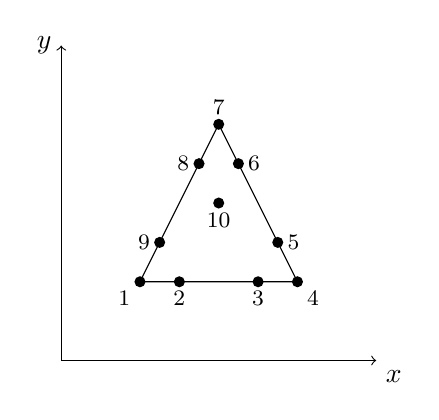
\begin{tikzpicture}
\draw[->] (0,0) -- (4,0) node[below right] {$x$};
\draw[->] (0,0) -- (0,4) node[left] {$y$};
\draw (1,1) -- (3,1) -- (2,3) -- cycle;
\fill (1,1) circle(2pt) node[below left] {\footnotesize1};
\fill (1.5,1) circle(2pt) node[below] {\footnotesize2};
\fill (2.5,1) circle(2pt) node[below] {\footnotesize3};
\fill (3,1) circle(2pt) node[below right] {\footnotesize4};
\fill (2.75,1.5) circle(2pt) node[right] {\footnotesize5};
\fill (2.25,2.5) circle(2pt) node[right] {\footnotesize6};
\fill (2,3) circle(2pt) node[above] {\footnotesize7};
\fill (1.75,2.5) circle(2pt) node[left] {\footnotesize8};
\fill (1.25,1.5) circle(2pt) node[left] {\footnotesize9};
\fill (2,2) circle(2pt) node[below] {\footnotesize10};
\end{tikzpicture}
\end{center}

$\varphi = \alpha_1 + \alpha_2 x + \alpha_3y + \alpha_4x^2 + \alpha_5xy+ \alpha_6y^2 + \alpha_7x^3 + \alpha_8x^2y + \alpha_9xy^2 + \alpha_{10}xy^2 = N_i\Phi_i= [N]\{\Phi\},\ i = 1,\dots, 10$.

\newpage

Функции формы для квадратичных треугольных конечных элементов в $L$-координатах:

\begin{center}
\begin{tabular}{cc}
	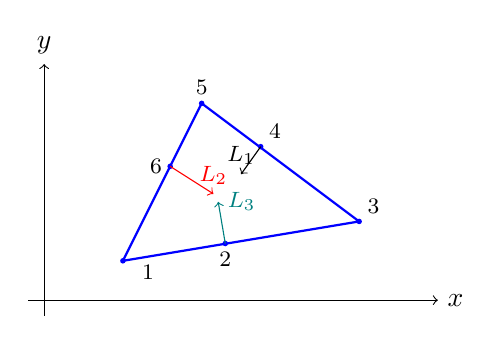
\begin{tikzpicture}
    		\draw[->] (-0.2,0) -- (5,0) node[right] {$x$};
    		\draw[->] (0,-0.2) -- (0,3) node[above] {$y$};
   		\draw[blue, thick] (1,0.5) -- (4,1) -- (2,2.5) -- cycle;
		{\footnotesize
   	 	\node at (1.5,0.55) [below left] {$1$};
   		\node at (4,1) [above right] {$3$};
    		\node at (2,2.5) [above] {$5$};
		\node at (2.3, 0.72)[below] {$2$};
		\node at (1.6, 1.7)[left] {$6$};
		\node at (2.75, 1.95)[above right] {$4$};
		}
		\fill[blue] (1, 0.5) circle (1pt);
		\fill[blue] (4,1) circle (1pt);
		\fill[blue] (2,2.5) circle (1pt);
		\fill[blue] (2.3, 0.72) circle (1pt);
		\fill[blue] (1.6, 1.7) circle (1pt);
		\fill[blue] (2.75, 1.95) circle (1pt);

		\draw[->][thin, teal] (2.3, 0.72) -- (2.21,1.25) node[right] {\footnotesize $L_3$};
		\draw[->][thin, red] (1.6, 1.7) -- (2.15,1.35) node[above] {\footnotesize $L_2$};
		\draw[->][thin] (2.75, 1.95) -- (2.5,1.6) node[above] {\footnotesize $L_1$};
	\end{tikzpicture}

& 

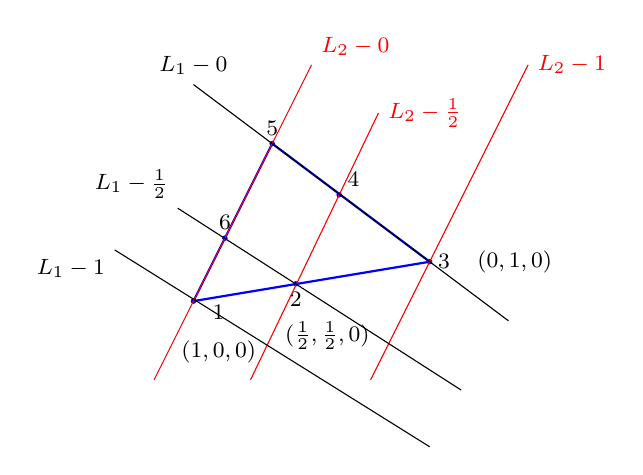
\begin{tikzpicture}
   		\draw[blue, thick] (1,0.5) -- (4,1) -- (2,2.5) -- cycle;
		{\footnotesize
   	 	\node at (1.5,0.55) [below left] {$1$};
		\node at (1.9, 0.1)[below left] {$(1,0,0)$};
   		\node at (4,1) [right] {$3$};
		\node at (4.5, 1)[right] {$(0,1,0)$};
    		\node at (2,2.5) [above] {$5$};
		\node at (2.3, 0.72)[below] {$2$};
		\node at (2.7, 0.35)[below] {$\footnotesize(\frac{1}{2},\frac{1}{2},0)$};
		\node at (1.4, 1.3)[above] {$6$};
		\node at (2.85, 1.85)[above right] {$4$};
		}
		\fill[blue] (1, 0.5) circle (1pt);
		\fill[blue] (4,1) circle (1pt);
		\fill[blue] (2,2.5) circle (1pt);
		\fill[blue] (2.3, 0.72) circle (1pt);
		\fill[blue] (1.4, 1.3) circle (1pt);
		\fill[blue] (2.85, 1.85) circle (1pt);
		
		\draw[thin, red] (0.5,-0.5) -- (2.5, 3.5) node[above right] {\footnotesize $L_2 - 0$};
		\draw[thin, red] (1.725, -0.5) -- (3.35, 2.89) node[right] {\footnotesize $L_2 - \frac{1}{2}$};
		\draw[thin, red] (3.25,-0.5) -- (5.25, 3.5) node[right] {\footnotesize $L_2 - 1$};
		
		\draw[thin] (5,0.25) -- (1, 3.25) node[above] {\footnotesize $L_1 - 0$};
		\draw[thin] (4,-1.35) -- (0, 1.15) node[below left] {\footnotesize $L_1 - 1$};
		\draw[thin] (4.4, -0.63) -- (0.8, 1.68) node[above left] {\footnotesize $L_1 -  \frac{1}{2}$};
	\end{tikzpicture}
	\\
\end{tabular}
\end{center}
\[N_1 = L_1 \left(L_1 - \frac{1}{2}\right)\]

(нужно взять такие линии, которые захватывают все узлы, кроме первого)

Нормируем:
\[N_1 = \frac{L_1 \left(L_1 - \displaystyle\frac{1}{2}\right)}{1 \left(1 - \displaystyle\frac{1}{2}\right)} = L_1 (2L_1 - 1)\]
\[N_2 = \frac{L_2L_1}{\displaystyle\frac{1}{2} \cdot \frac{1}{2}} = 4L_1L_2\]
\[N_3 = \frac{L_2 \left(L_2 - \displaystyle\frac{1}{2}\right)}{1 \left(1 - \displaystyle\frac{1}{2}\right)} = L_2 (2L_2 - 1)\]
\[N_4 = 4L_2L_3\]
\[N_5 = L_3(2L_3 - 1)\]
\[N_6 = 4L_1L_3\]
\[N_{\beta} = \prod_{\delta=1}^n \frac{F_{\delta}}{F_{\delta} |_{L_1,L_2,L_3}},\ F_{\delta} - \text{ пробные функции}\]
